\documentclass[11pt, twocolumn]{article}
\usepackage{microtype}
\usepackage{graphicx}

\begin{document}

\title{Transformers for Semi-Supervised Agents}

\author{Peter Lovett}

\maketitle

\section{Introduction}

The rapid ascension of transformer neural networks calls into question the limit of their application. Their ubiquitous presence in natural language processing shows their ability to capture complex patterns (whether it captures the patterns we want it to is still debated). Many of these methods pre-train their transformer networks on large unsupervised datasets before fine-tuning them on a target task. These methods have been adapted to images but not yet extensively on agent-environment tasks.

Environments can be complex and demanding for learning algorithms. Some environments require the model to approximate gravity, learn motion controls, and recognize sub-goals. To make the final task easier, semi-supervised and unsupervised methods have been employed to more quickly acclimate a model to its environment. These pre-training sequences hope that by cheaply training the model on unlabeled data, the model will learn functions that can be reused on the final task.

This work explores the use of pre-trained transformers for agent-environment tasks. By comparing  transformer networks to other pre-training methods for agent-environment tasks we try to gain a better understanding of their qualities and deficiencies. Using our results we try to evaluate how effective pre-trained transformers are for agent-environment tasks.

\section{Method}

The method section has two pieces, the Deep Q-Learning algorithm\cite{mnih2013playing} applied to our setting and the pretraining process. 

\subsection{Deep Q-Learning}
In the agent-environment task framework and algorithm controls an agent that is trying to maximise some reward in an environment. This broadly fits many different real world tasks, which makes it convenient for analysis. The original Q-Learning algorithm \cite{watkins1992q} was effective for discrete environments and actions, but required storage of information about all possible states. The algorithm was intractable for large state spaces. When renewed interest in deep learning proved the effectiveness of large neural networks as universal function approximators, the deep Q-Learning algorithm was devised.

In order for a model to effectively choose the best actions it needs to understand the relative value of its choices. Formally, give state $s_t$ and possible actions , choose the action $a_t$ that maximises the sum of future rewards for this episode. The deep Q-Learning algorithm attempts to approximate a function from state, action pairs to future values. 

\begin{equation}
a_t = max_a Q (s_t, \alpha, \theta)
\end{equation}

In our setting we use the $CartPole-v0$ environment from the OpenAI Gym \cite{brockman2016openai}. This is a simple environment, where given information about the angle and position of a pole attached to a cart, the agent must balance the pole upright for as long as possible. We choose to stop the cart if it successfully balances the pole for 200 time steps. Our goal is to train a neural network to approximate the value of moving in either direction to balance the cart. To make the task easier for our final model, we pretrain a network to feed into the final model.

\subsection{Pretraining}
The dynamics of the environment are unknown to the model when it is randomly initialized. This means that before the model can understand the value of making a certain move, it must understand the impact of making certain actions. Ideally, we want a model that already has the intuitive grasp of physics that humans possess. We attempt to close this gap by pretraining a neural network on offline episodes from the same environment. The pretrained model should capture the dynamics of the environment, simplifying value function approximator's task. This should lead to improved task performance and faster convergence for the value function approximator.

Offline episodes are created by randomly sampling a possible action and recording the observations from the environment. We collect 2000 episodes of up to 200 frames as our training database. We train a transformer model to predict the next time step given all previous time steps. This is a regression problem on four continuous values, so we use the mean square error between our estimations and the real values to train the model. Figure \ref{fig:diagram} contains a depiction of the model used. The first and last feedforward layers in the model map the input from the hidden size to the observation size and vice versa. During testing, the last hidden layer is ignored and the full hidden vector is returned as a representation of the environment's state. Our baseline is a simple RNN model followed by two feedforward layers seperated by a ReLU activation. The baseline follows an identical procedure during test time. Each model is trained for 20 epochs using stochastic gradient descent with a learning rate of $1e-3$. After 20 epochs the loss appears to plateau on both the training and evaluation data.

\begin{figure}
\begin{center}
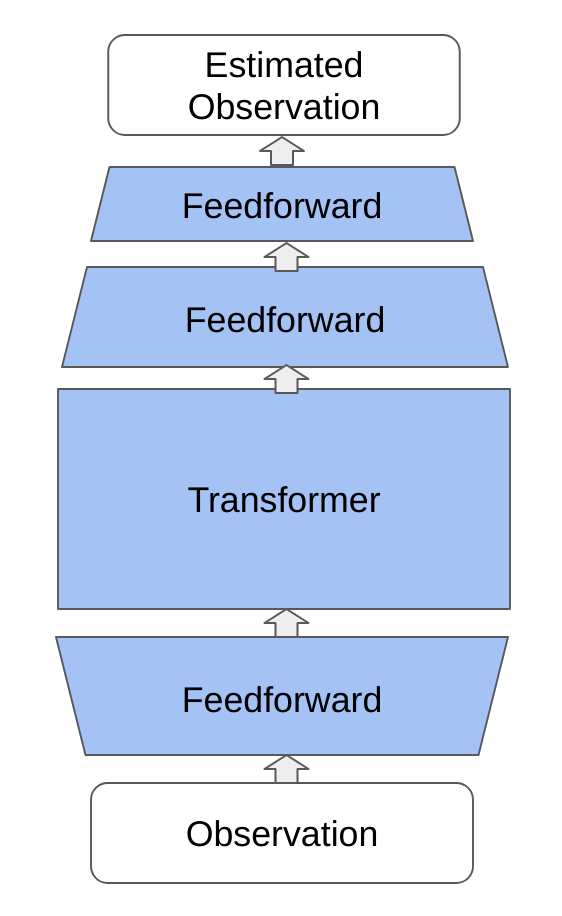
\includegraphics[scale=0.25]{model_diagram.png}
\caption{The transformer model used for observation prediction. Here the two white layers are the input and output, while the blue layers are the model itself. All layers except for the last feedforward layer were used at test time.}
\label{fig:diagram}
\end{center}
\end{figure}


\section{Results}
To evaluate the pretrained models impact on the deep Q-Learning setting, we set up a simple two layer feedforward network on top of the pretrained models. This model is trained using the deep Q-Learning algorithm to maximize the reward obtained by our agent. The network is trained using batches of 128 state-action pairs, a $\gamma$ of $0.999$, $\epsilon$ starting at 0.9 and decaying to 0.05 in 200 steps. The target network is updated every 10 training steps. The replay memory queue contains 1,000,000 state-action pairs. 

\begin{figure}
\begin{center}
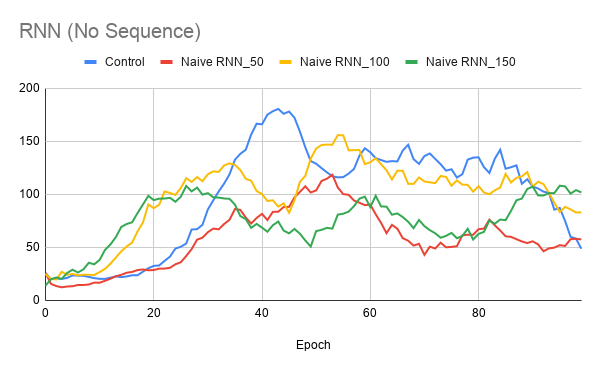
\includegraphics[scale=0.35]{naive_rnn.png}
\caption{This chart displays the results of using an RNN to encode the relevant information in the environment with varying embedding sizes. Here the y-axis is the trailing average for the total reward from the last 100 episodes.}
\label{fig:naive_rnn}
\end{center}
\end{figure}

\begin{figure}
\begin{center}
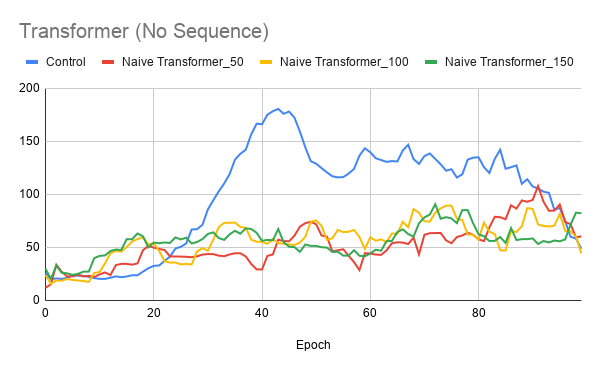
\includegraphics[scale=0.35]{naive_transformer.png}
\caption{This chart displays the results of using a Transformer to encode the relevant information in the environment with varying embedding sizes. Here the y-axis is the trailing average for the total reward from the last 100 episodes.}
\label{fig:naive_transformer}
\end{center}
\end{figure}

Our results fall into two categories, the setting where the pretrained model gets only the current observation and the setting where the model gets all previous observations in this episode. Figure \ref{fig:naive_rnn} displays the trailing average of reward for the baseline pretrained RNN. Figure \ref{fig:naive_transformer} displays the trailing average of reward for the transformer model. The trailing average is used to limit the variance displayed. Figures \ref{fig:smart_rnn} and \ref{fig:smart_transformer} show the performance of the two methods when given all previous data. These two methods should display stronger performance as they can encode information about momentum and previous states more effectively. 

\begin{figure}
\begin{center}
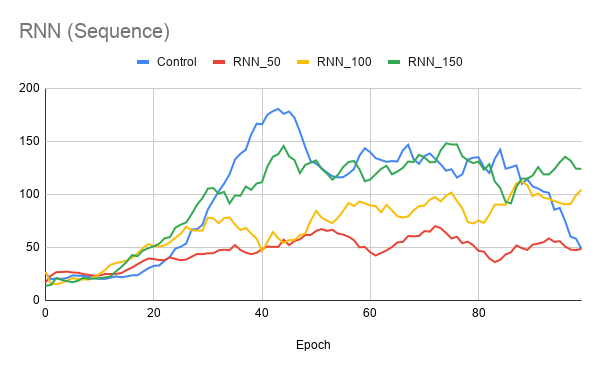
\includegraphics[scale=0.35]{smart_rnn.png}
\caption{This chart displays the results of using an RNN to encode the relevant information in the environment with varying embedding sizes. Here the y-axis is the trailing average for the total reward from the last 100 episodes.}
\label{fig:smart_rnn}
\end{center}
\end{figure}

\begin{figure}
\begin{center}
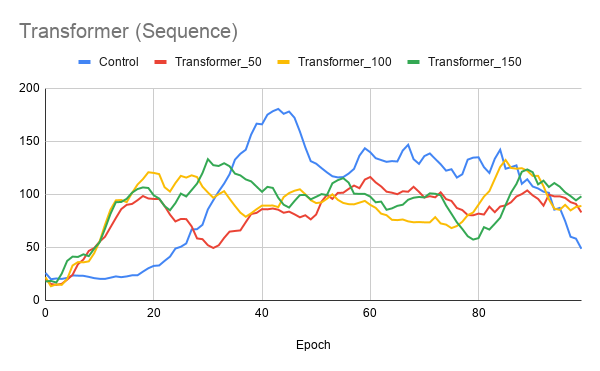
\includegraphics[scale=0.35]{smart_transformer.png}
\caption{This chart displays the results of using a Transformer to encode the relevant information in the environment with varying embedding sizes. Here the y-axis is the trailing average for the total reward from the last 100 episodes.}
\label{fig:smart_transformer}
\end{center}
\end{figure}


\section{Discussion}
The results are unimpressive. While the models seem to quickly jump the performance of the algorithm, they seem to plateau, bringing in to question the utility of the pretraining method. The RNN model with no sequence data has similar performance to the transformer model with sequential data. The RNN does not seem to require as much sequential data as the transformer in order to properly encode the environment data. This is surprising and I would have predicted the opposite. The transformer mainly uses attention so limiting the size of the data it can use likely reduces the utility of the learned attention weights. There seems limited effectiveness gained through increasing the dimensionality of the pretrained models. The only model that has a clear dimensionality performance relationship is the RNN with sequential data. The high noise of the Q-Learning training process seems to drown out any improvement that dimensionality could supply in the other models.

The issues with the pretrained models are not immediately obvious and would require further experimentation to understand. The models could have overfit the training data but they seemed to also be decreasing the evaluation loss. Potentially the 20 epochs the models were trained for were too short. Longer training times could fix the issues with instable reward values during the deep Q-Learning phase. When it comes to machine learning there are always more experiments that can be run.	

\bibliography{proposal}
\bibliographystyle{abbrv}
\end{document}
